
\documentclass[letterpaper, reqno,11pt]{article}
\usepackage[margin=1.0in]{geometry}
\usepackage{color,latexsym,amsmath,amssymb}
\usepackage{fancyhdr}
\usepackage{amsthm}
\usepackage{mathtools}
\usepackage{tikz}
\usepackage{float}
\usepackage{centernot}
\usepackage{subcaption}
\usepackage{extarrows}
\usetikzlibrary{hobby}
\usetikzlibrary{shapes.multipart}
\usepackage{pgfplots}
\pgfplotsset{compat=1.7}
\usetikzlibrary{arrows.meta}
\usepackage{cancel}
\usetikzlibrary{decorations.markings}
\usetikzlibrary{shapes}
\usetikzlibrary{arrows}
\usepgfplotslibrary{fillbetween}
\usetikzlibrary{patterns}

\newcommand{\RR}{\mathbb{R}}
\newcommand{\CC}{\mathbb{C}}
\newcommand{\ZZ}{\mathbb{Z}}
\newcommand{\QQ}{\mathbb{Q}}
\newcommand{\NN}{\mathbb{N}}
\def\upint{\mathchoice%
  {\mkern13mu\overline{\vphantom{\intop}\mkern7mu}\mkern-20mu}%
  {\mkern7mu\overline{\vphantom{\intop}\mkern7mu}\mkern-14mu}%
  {\mkern7mu\overline{\vphantom{\intop}\mkern7mu}\mkern-14mu}%
  {\mkern7mu\overline{\vphantom{\intop}\mkern7mu}\mkern-14mu}%
  \int}
\def\lowint{\mkern3mu\underline{\vphantom{\intop}\mkern7mu}\mkern-10mu\int}
\DeclareMathOperator{\card}{card}
\DeclareMathOperator{\Binomial}{Binomial}
\DeclareMathOperator{\Span}{span}
\pagestyle{fancy}
\lhead{Math 321 Lecture 25}
\rhead{Yuchong Pan}
\begin{document}
\pagenumbering{arabic}
\title{Math 321 Lecture 25}
\author{Yuchong Pan}
\date{March 8, 2019}
\newtheorem{thm}{Theorem}
\newtheorem{defn}{Definition}
\newtheorem*{remark}{Remark}
\newtheorem{claim}{Claim}
\newtheorem{cor}{Corollary}
\newtheorem{lemma}{Lemma}
\newtheorem{prop}{Proposition}
\newtheorem{fact}{Fact}
\maketitle
%

\section{Uniform Convergence and Non-Convergence of Fourier Series}

\begin{figure}[H]
  \centering
  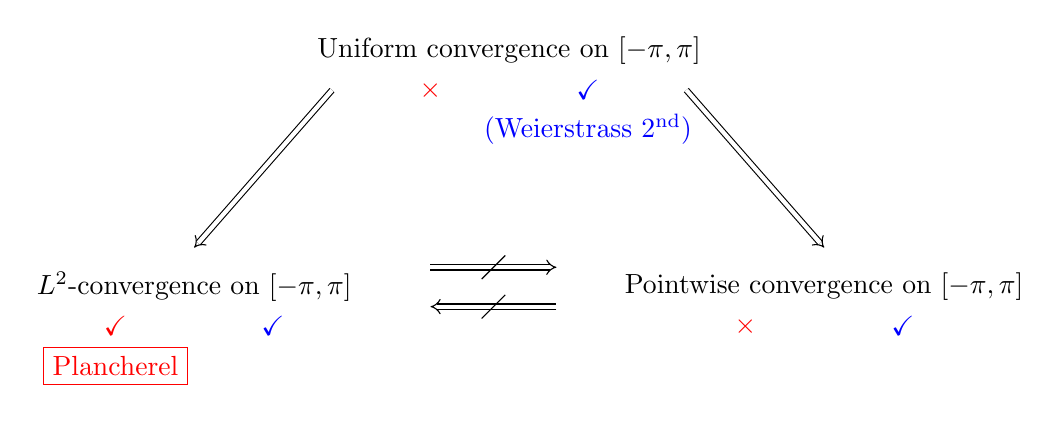
\begin{tikzpicture}
    \node at (0, 0) {Uniform convergence on $[-\pi, \pi]$};
    \node at (-4, -3) {$L^2$-convergence on $[-\pi, \pi]$};
    \node at (4, -3) {Pointwise convergence on $[-\pi, \pi]$};
    \draw[-implies, double equal sign distance] (-2.25, -0.5) -- (-4, -2.5);
    \draw[-implies, double equal sign distance] (2.25, -0.5) -- (4, -2.5);
    \draw[-implies, double equal sign distance] (-1, -2.75) -- (0.6, -2.75);
    \draw[-implies, double equal sign distance] (0.6, -3.25) -- (-1, -3.25);
    \draw (-0.35, -2.9) -- (-0.05, -2.6);
    \draw (-0.35, -3.4) -- (-0.05, -3.1);
    \node at (-1, -0.5) {\color{red} $\times$};
    \node at (1, -0.5) {\color{blue} $\checkmark$};
    \node at (1, -1) {\color{blue} (Weierstrass $2^\text{nd}$)};
    \node at (-5, -3.5) {\color{red} $\checkmark$};
    \node at (-3, -3.5) {\color{blue} $\checkmark$};
    \node at (-5, -4) {\color{red} \fbox{Plancherel}};
    \node at (3, -3.5) {\color{red} $\times$};
    \node at (5, -3.5) {\color{blue} $\checkmark$};
  \end{tikzpicture}
\end{figure}

\begin{enumerate}
  {\color{red} \item How does the Fourier series of $f \in \mathcal C^{2\pi}$ interact with these different notions of convergence?}
  {\color{blue} \item Does there exist a sequence of trignometric polynomials $P_n$ such that $P_n \to f \in \mathcal C^{2\pi}$?}
\end{enumerate}

\subsection{Dirichlet and Fej\'er Kernels}

Recall:
\begin{align*}
  s_N f(x) &= \text{$N^\text{th}$ partial Fourier series of $f$} = \sum_{k = -N}^N \widehat f(k) e^{ikx} \\
  &\xlongequal[\text{Problem 5}]{\text{HW 8}} f * D_N(x), \qquad \text{where} \\
  \Aboxed{D_N(x) &= \sum_{k = -N}^N e^{ikx} = \frac{\sin\left[\left(N + \frac{1}{2}\right) x\right]}{\sin\left(\frac{x}{2}\right)}} : \text{Dirichlet kernel}, \\
  f * g(x) &= \frac{1}{2\pi} \int_{-\pi}^\pi f(x - t) g(t) dt.
\end{align*}

\begin{thm}
  \normalfont
  \begin{enumerate}
  \item $D_N$ is a trignometric polynomial by definition.
  \item $\frac{1}{2\pi} \int_{-\pi}^\pi D_N(x) dx = 1$ for all $N \geq 0$ [because $\int_{-\pi}^\pi D_N(x) dx = \sum_{k = -N}^N \underbrace{\int_{-\pi}^\pi e^{ikx} dx}_{\tiny \left\{\begin{array}{ll} 0, & \forall k \in \ZZ \setminus \{ 0 \}, \\ 2\pi, & k = 0. \end{array}\right.} = 2\pi$].
  \item There exist absolute constants $c_1, c_2 > 0$ such that for all $N \geq 1$,
    \[ \boxed{c_1 \log N \overset{\text{(*)}}{\leq} \frac{1}{2\pi} \int_{-\pi}^\pi |D_N(x)| dx \leq c_2 \log N} \Rightarrow \sup_N \lVert D_N \rVert_1 = \infty. \]
  \end{enumerate}
\end{thm}

\noindent {\bf Recall:}
\begin{align*}
  \sigma_N f(x) &= \frac{1}{N} [s_1 f(x) + s_2 f(x) + \ldots + s_N f(x)] \\
  &= \text{$N^\text{th}$ partial Ces\`aro sum of $f$} = f * K_N(x).
\end{align*}

\noindent {\bf Moral:} $\sigma_N f$ has a better chance of converging than $s_N f$.
\begin{align*}
  \{ a_N \}: & \quad a_1 = 1, \quad a_2 = -1, \quad a_3 = 1, \quad a_4 = -1, \quad \ldots. \\
  \{ s_N \}: & \quad s_1 = a_1 = 1, \quad s_2 = a_1 + a_2 = 0, \quad s_3 = a_1 + a_2 + a_3 = 1, \quad s_4 = 0, \quad \ldots && \text{$\lim_N s_N$ does not exist}. \\
  \{ \sigma_N \}: & \quad \sigma_1 = s_1 = 1, \quad \sigma_2 = \frac{1}{2}(s_1 + s_2) = \frac{1}{2}, \quad \sigma_3 = \frac{1}{3}(s_1 + s_2 + s_3) = \frac{2}{3}, \quad \ldots && \lim_N \sigma_N = 1.
\end{align*}

\noindent In HW 8, we saw:
\[ K_N(t) = \frac{\sin^2\left(\frac{Nt}{2}\right)}{2N \sin^2\left(\frac{t}{2}\right)} = \frac{1}{N} (D_1(t) + \ldots + D_N(t)). \]

\begin{thm}[Fej\'er]
  \normalfont
  \begin{enumerate}
  \item \label{enum:1} $K_N$ is a trignometric polynomial.
  \item $\frac{1}{2\pi} \int_{-\pi}^\pi K_N(x) dx = 1$ (because $\frac{1}{2\pi} \int_{-\pi}^\pi K_N(x) dx = \frac{1}{N} \sum_{k = 1}^N \frac{1}{2\pi} \int_{-\pi}^\pi D_k(x) dx = \frac{1}{N} \underbrace{(1 + \ldots + 1)}_\text{$N$ times} = 1$).
  \item $\frac{1}{2\pi} \int_{-\pi}^\pi|K_N(x)| dx = 1$ for any $N$ $\Rightarrow$ $\sup_N \lVert K_N \rVert_1 = 1 < \infty$.
  \item \label{enum:4} For every $\delta > 0$, $\int_{|x| > \delta} K_N(x) dx \xrightarrow{N \to \infty} 0$.

    \begin{figure}[H]
      \centering
      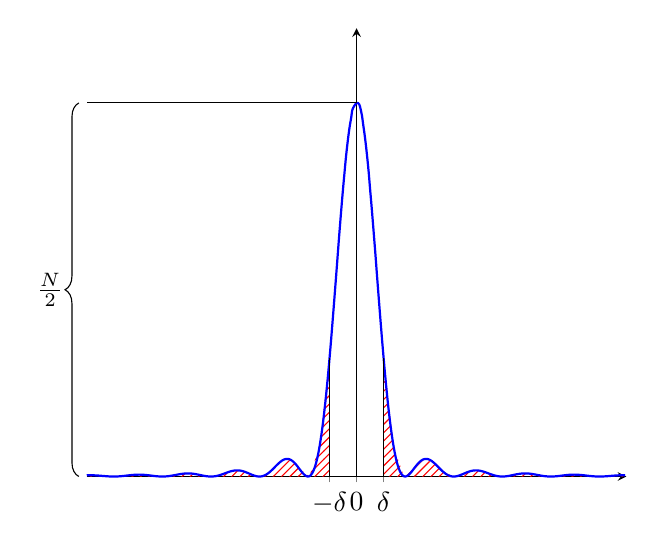
\begin{tikzpicture}[
          declare function={f(\x)=(\x!=0)*(sin(50*\x)^2)/(200*sin(\x/2)^2)+(\x==0)*50;}
        ]
        \begin{axis}[
            xmin=-20,
            xmax=20,
            ymin=0,
            ymax=60,
            xtick={0, -2, 2},
            xticklabels={$0$, $-\delta$, $\delta$},
            ymajorticks=false,
            axis x line=bottom,
            axis y line=center,
            clip=false,
          ]
          \addplot[thick, blue, samples at={-20, -19.9, ..., -0.2, 0, 0.2, 0.3, ..., 20}, smooth](x,{f(x)});
          \addplot[name path=zero-left, draw=none, domain={-20:-2}] {0};
          \addplot[name path=left, draw=none, domain={-20:-2}] {f(x)};
          \addplot[name path=zero-right, draw=none, domain={2:20}] {0};
          \addplot[name path=right, draw=none, domain={2:20}] {f(x)};
          \draw (axis cs:-2, 0) -- (axis cs:-2, {f(-2)});
          \draw (axis cs:2, 0) -- (axis cs:2, {f(2)});
          \draw (axis cs:0, 50) -- (axis cs:-20, 50);
          \draw[decoration={brace, raise=0.1cm, amplitude=5pt}, decorate] (axis cs:-20, 0) -- (axis cs:-20, 50) node[midway, left, xshift=-5pt] {$\frac{N}{2}$};
          \addplot[pattern=north east lines, pattern color=red] fill between[of=left and zero-left];
          \addplot[pattern=north east lines, pattern color=red] fill between[of=right and zero-right];
        \end{axis}
      \end{tikzpicture}
    \end{figure}
  \end{enumerate}
\end{thm}

\begin{cor}
  \normalfont Use Fej\'er's theorem \ref{enum:1} -- \ref{enum:4} to show that for every $f \in \mathcal C^{2\pi}$,
  \[ \frac{1}{2\pi} \int_{-\pi}^\pi f(x-y) K_N(y) dy = f * K_N = \sigma_N f \xrightarrow{N \to \infty} f \; \text{uniformly}. \]
\end{cor}

\begin{proof}[Proof of (*)]
  ~
  
  \begin{figure}[H]
    \centering
    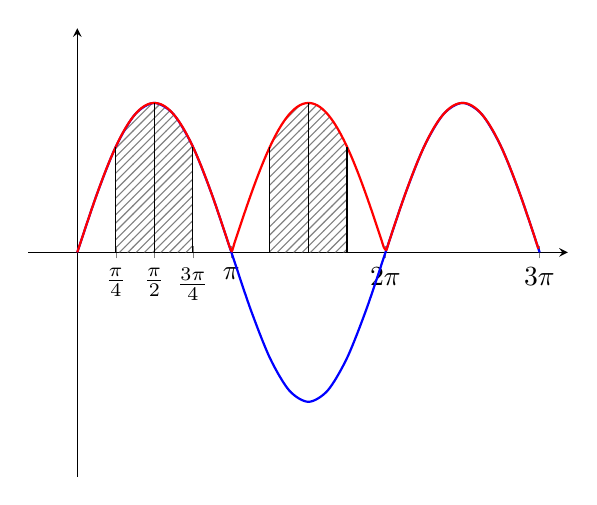
\begin{tikzpicture}
      \begin{axis}[
          xmin=-1,
          xmax=10,
          ymin=-1.5,
          ymax=1.5,
          xtick={0.785, 1.57, 2.355, 3.14, 6.28, 9.42},
          xticklabels={$\frac{\pi}{4}$, $\frac{\pi}{2}$, $\frac{3\pi}{4}$, $\pi$, $2\pi$, $3\pi$},
          ymajorticks=false,
          axis x line=center,
          axis y line=center,
        ]
        \addplot[thick, blue, domain={0:3*pi}, smooth](x,{sin(x/pi*180)});
        \addplot[name path=abssin, thick, red, samples at={0, 0.05, ..., 9.45}, smooth](x,{abs(sin(x/pi*180))});
        \draw (axis cs:pi/4, 0) -- (axis cs:pi/4, {abs(sin(180/4))});
        \draw (axis cs:pi/2, 0) -- (axis cs:pi/2, {abs(sin(180/2))});
        \draw (axis cs:3/4*pi, 0) -- (axis cs:3/4*pi, {abs(sin(3/4*180))});
        \draw (axis cs:5/4*pi, 0) -- (axis cs:5/4*pi, {abs(sin(5/4*180))});
        \draw (axis cs:3/2*pi, 0) -- (axis cs:3/2*pi, {abs(sin(3/2*180))});
        \draw (axis cs:7/4*pi, 0) -- (axis cs:7/4*pi, {abs(sin(7/4*180))});
        \addplot[name path=zero, draw=none, domain={0:10}] {0};
        \addplot[pattern=north east lines, pattern color=gray] fill between[of=abssin and zero, soft clip={domain=pi/4:3/4*pi}];
        \addplot[pattern=north east lines, pattern color=gray] fill between[of=abssin and zero, soft clip={domain=5/4*pi:7/4*pi}];
      \end{axis}
    \end{tikzpicture}
  \end{figure}

  Note that
  \[ \sin\left(\frac{x}{2}\right) \leq Cx, \qquad x \in [-\pi, \pi], \]
  and that
  \[ \frac{k\pi}{2} - \frac{\pi}{4} \leq \left(N + \frac{1}{2}\right) \frac{x}{2} \leq \frac{k\pi}{2} + \frac{\pi}{4} \text{ for some odd integer $k$}. \]
  Therefore, we have
  \[ \int_{-\pi}^\pi \left|\frac{\sin\left[\left(N + \frac{1}{2}\right) x\right]}{\sin\left(\frac{x}{2}\right)}\right| dx \geq \sum_{\substack{\text{$k$ odd integer} \\ k \leq N}} \int_{\frac{k\pi}{2} - \frac{\pi}{4}}^{\frac{k\pi}{2} + \frac{\pi}{4}} \frac{c_0}{|x|} dx \geq c_0 \sum_{\substack{\text{$k$ odd integer} \\ k \leq N}} \frac{1}{k} \geq c_1 \log N. \]
\end{proof}

\end{document}
